\chapter{Metodologia}

    % Como discutido anteriormente, as diferentes formas nas quais os dados censitários, bem como o de outras pesquisas como a Pesquisa Nacional por Amostra de Domicílios (PNAD), se diferem basicamente por seu formato, JSON para a API e 
    
    % Por conta das diferentes formas em que os dados se encontram disponibilizados pelo IBGE discutidas anteriormente, e também pelo caráter dos mesmos quanto à granularidade e quais dados são disponibilizados, foram tomadas duas diferentes abordagens: a de coletar os dados através da API de serviço de dados e a de baixar os arquivos de microdados dos Censos de 2000 e 2010 e transformá-los em dados 

    Como discutido anteriormente, as diferentes formas nas quais os dados censitários, bem como de outras pesquisas do IBGE, são disponibilizados, se diferem basicamente quanto ao seu grão e formato, sendo os agregados disponibilizados via API no formato JSON, enquanto os microdados em arquivos de texto em um formato compactado que será explicado em detalhes na seção \ref{sec-microdados}. Dessa forma, duas diferentes abordagens foram tomadas no decorrer do desenvolvimento do trabalho: a de coletar os dados através da API e a de baixar os arquivos de microdados do IBGE e processá-los para então criar os conjuntos de dados disponíveis no repositório.
    

\section{APIs do serviço de dados do IBGE}
\label{metodoslogia-API}

    O IBGE oferece ao todo 17 APIs em seu serviço de dados, incluindo a de Agregados, citada anteriormente, a de Localidades, que inclui os códigos dos vários níveis de localidade (p. ex. unidade federativa (UF), macrorregião, município), a de Metadados, incluindo informações como periodicidade e variáveis disponíveis em cada uma das pesquisas disponíveis na API, entre outras. Nestas APIs é possível, através de \textit{Uniform Resource Locators} (URLs) gerar requisições por meio de bibliotecas como a \textit{requests} do \textit{python} para obter os dados da API no formato \textit{Javascript Object Notation} (JSON). Por exemplo, ao fazer uma requisição à API de localidades utilizando o URL \url{servicodados.ibge.gov.br/api/v1/localidades/distritos} obteremos uma lista de valores no formato exemplificado em \textit{Listing} \ref{lst:exemplo-api-localidades}:

\begin{lstlisting}[float = h, label={lst:exemplo-api-localidades},language=Python, caption=Exemplo de resultado de uma requisição da API de localidades.]
{"id":421400310, "nome":"Mirador",
  "municipio":{"id":4214003,"nome":"Presidente Getúlio",
    "microrregiao":{"id":42011,"nome":"Rio do Sul",
      "mesorregiao":{"id":4204,"nome":"Vale do Itajaí",
        "UF":{"id":42, "sigla":"SC","nome":"Santa Catarina",
          "regiao":{"id":4, "sigla":"S", "nome":"Sul"}}}},
    "regiao-imediata":{"id":420023, "nome":"Ibirama - Presidente Getúlio",
      "regiao-intermediaria":{"id":4207, "nome":"Blumenau",
          "regiao":{"id":4, "sigla":"S","nome":"Sul"}}}}
}
\end{lstlisting}

% {"id":420690010, "nome":"Dalbérgia",
%   "municipio":{"id":4206900, "nome":"Ibirama",
%     "microrregiao":{"id":42011, "nome":"Rio do Sul", "mesorregiao":{"id":4204, "nome":"Vale do Itajaí",
%         "UF":{"id":42, "sigla":"SC", "nome":"Santa Catarina",
%           "regiao":{"id":4, "sigla":"S", "nome":"Sul"}}}},
%     "regiao-imediata":{"id":420023, "nome":"Ibirama - Presidente Getúlio",
%       "regiao-intermediaria":{"id":4207, "nome":"Blumenau",
%         "UF":{"id":42, "sigla":"SC", "nome":"Santa Catarina",
%           "regiao":{"id":4, "sigla":"S", "nome":"Sul"}}}}}}

    Por mais que a formatação JSON tenha uma praticidade maior em um ponto de vista transacional ou orientado à objetos, ele não é ideal para o uso analítico por conta de uma certa complexidade intrínseca para a navegação pelos dados e necessitando de certo trabalho para a interpretação dos mesmos. 
    
    Dado que normalização não é uma prioridade quando se trata de análise, mas sim a simplicidade de na hora de se criarem consultas, foi aplicado à \textit{string} de resultados da requisição um processo de \textit{unnesting} (em português desaninhamento), cujo algoritmo se encontra no \textit{listing} \ref{lst:unnesting} do apêndice \ref{apend-code}. Tal processo é o oposto do conceito conhecido por \textit{nesting} e consiste de, recursivamente, subir o nível de aninhamento (\textit{nesting-level}) de uma entrada, para o nível de seu nível imediatamente superior, até que todos os valores estejam alinhados.

    Por exemplo, aplicando o algoritmo de \textit{unnesting} juntamente com a função \verb|make_df()| (\textit{listing} \ref{apend-code}.\ref{lst:make-df}), gera um \textit{DataFrame} como a tabela \ref{tab:exemplo-api-localidades}, com todos os dados em um mesmo \textit{nesting-level}.

\begin{center}
    \begin{table}[ht]
        \begin{tabular}{c l c l c l}
            \hline
                id-distrito & nome-distrito & id-municipio & nome-municipio & $\dotsi$ & nome-regiao\\
            \hline
                421400310 & Mirador & 4214003 & Presidente Getúlio & $\dotsi$ & Sul\\
                420690010 & Dalbérgia & 4206900 & Ibirama & $\dotsi$ & Sul\\     
            \hline
        \end{tabular}
        \caption{Exemplo dos dados de localidade em formato tabular. Fonte: Dados do autor (2023).}
        \label{tab:exemplo-api-localidades}
    \end{table}
\end{center}

    Um certo problema que pode ainda ocorrer é que, mesmo após o \textit{unnesting}, os dados em JSON podem conter também elementos em formato de lista, gerando assim uma coluna na tabela de resultado que possui em si uma lista de valores. Portanto se faz necessário um segundo tratamento para estes casos, que é facilmente resolvido armazenando o conjunto de dados dentro de um objeto do tipo \textit{DataFrame} da biblioteca \textit{pandas} da linguagem \textit{python} e utilizar o método \lstinline{pandas.DataFrame().explode()}\footnote{Documentação disponível em <\url{pandas.pydata.org/docs/reference/api/pandas.DataFrame.explode.html}>, código fonte disponível em <\url{github.com/pandas-dev/pandas/blob/v2.1.1/pandas/core/frame.py\#L9432-L9558}>. Acessado em 30 de set. 2023.}     de modo a converter elementos \textit{list-like} que possam existir dentro das colunas em linhas, copiando os demais valores, como é exemplificado pela figura \ref{fig:exploding-df}.

\begin{figure}[ht]
    \centering
    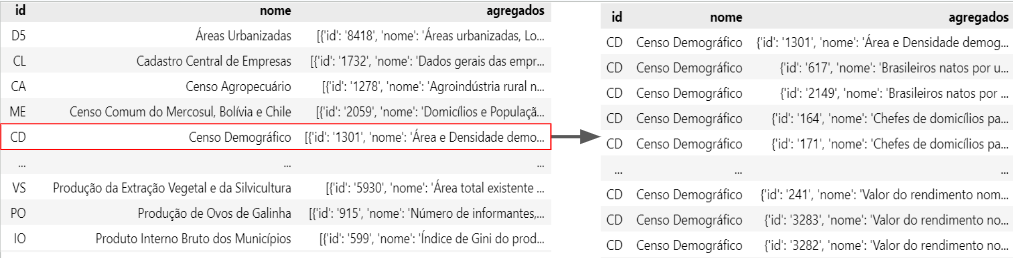
\includegraphics[width=\textwidth]{files/img/exploding_table.png}    \caption{Exemplo do uso do método \lstinline{pandas.DataFrame().explode()}. Fonte: Dados do autor (2023).}
    \label{fig:exploding-df}
\end{figure}

    Nota-se que os valores ``explodidos'' continuam aninhados, portanto nesse caso foi necessário reaplicar a função \lstinline{unnest_json()} de modo a separar adequadamente os dados. O processo completo é uma sequência de aplicação dessas duas funções conforme o necessário até termos um \textit{DataFrame} completamente desaninhado.

    Das 17 APIs disponíveis, foram carregados dados das APIs de localidades, países, agregados e metadados. 
    
    A API de localidades retorna as informações referentes aos identificadores geográficos do país definidos pelo IBGE, utilizados para identificar a área na qual foram coletados em praticamente todas as pesquisas do órgão. Esse serviço de dados possui ao todo quatro possíveis requisições nas quais os dados são separados por distritos, subdistritos, região metropolitana e região integrada de desenvolvimento. Os conjuntos de dados derivados podem ser juntados entre si através do identificador mais específico presentes nelas, sendo o ID do distrito nas duas primeiras e o id do município nas outras duas.

    Contendo 34 indicadores socioeconômicos dos 193 países membros da Organização das Nações Unidas (ONU) a API de países é a única que não utiliza apenas dados coletados pelo próprio IBGE e que também possui traduções em Espanhol e Inglês. Como uma requisição comum solicita a especificação dos países e/ou das variáveis desejadas, a estratégia adotada foi primeiramente obter todos os códigos distintos de países para posteriormente realizar uma requisição para cada país contendo todos os possíveis indicadores e concatenando todos os resultados em um único conjunto de dados. O código completo pode ser encontrado no \textit{listing} \ref{apend-code}.\ref{lst:api-paises}.

    A carga mais elaborada foi a de agregados, onde foi necessário primeiramente selecionar os IDs dos agregados, totalizando 8442 agregados de 68 pesquisas, cada qual contendo diversas variáveis e séries temporais. Então, obtidos os identificadores, foram requisitados à API os metadados de cada pesquisa. Tendo os dados de nível e o ID do agregado foi então possível usar a URL `https://servicodados.ibge.gov.br/api/v3/agregados/
    \{agregado\}/variaveis?localidades=\{nivel\}[all]', onde \verb|{agregado}| e \verb|{nivel}| são parâmetros passados conforme os metadados obtidos. 
    
    O resultado da requisição acima, transformado em \textit{DataFrame} é o mostrado na figura \ref{fig:tabela-agregado-pt1}. A coluna mais importante é de resultados, que irá conter duas listas de valores: classificações, contendo metadados acerca da variável, e, novamente, resultados, que por sua vez também contem listas, mas dessa vez com as séries dos valores numéricos. 
    
    Aplica-se então o método \verb|explode()| ao \textit{DataFrame} até termos os valores das séries distribuídos em uma coluna por ano, que, para normalizar a tabela, é executado o método \verb|melt()| para criar-se uma coluna de período e outra de valor. O resultado final é um conjunto de dados com as colunas variável, unidade, id, nome e nível geográfico da localidade (p. ex. Município, UF, \textit{etc.}), ano e valor.

\begin{figure}[ht]
    \centering
    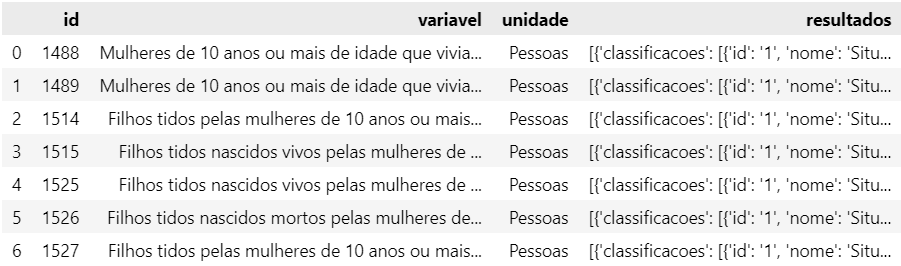
\includegraphics[width=\textwidth]{files/img/tabela_agregado_pt1.png}
    \caption{Tabela de dados após primeira requisição para a carga dos agregados. Fonte: Dados do Autor (2023).}
    \label{fig:tabela-agregado-pt1}
\end{figure}



    


\section{Microdados do Censo Demográfico}
\label{sec-microdados}

    Os dados fornecidos pela API de agregados consistem essencialmente na consolidação das respostas individuais de cada um dos entrevistados durante o processo de recenseamento de acordo com critérios locacionais, com seu menor grau de agregação sedo município. Tais informações são organizadas em um formato denominado pelo IBGE como microdados e são disponibilizados através do portal de produtos estatísticos da instituição\footnote{Para mais detalhes, consulte <\url{www.ibge.gov.br/estatisticas/todos-os-produtos-estatisticas.html}>. Acesso em 03 out. 2023}, estando disponibilizados em diversas pastas compactadas em formato \textit{.zip} que contém os arquivos de texto nos quais se encontram os dados. No entanto, os dados daqueles arquivos não estão imediatamente prontos para a utilização tal qual uma planilha ou um arquivo CSV, mas sim em um formato comprimido, onde os valores categóricos são codificados através de identificadores (IDs) numéricos, enquanto valores que originalmente possuíam casas decimais tem seus pontos flutuantes removidos. Dessa forma, os dados se apresentam conforme ilustrado pela figura \ref{fig:exemplo-microdado}:

\begin{figure}[ht]
    \centering
    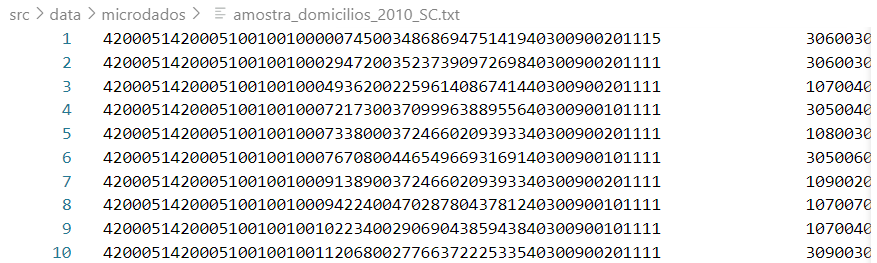
\includegraphics[width=\textwidth]{files/img/exemplo_microdado.png}
    \caption{Exemplo de microdados: primeiras 10 linhas da pesquisa de Domicílios do Censo de 2010 no estado de Santa Catarina. Fonte: Dados do Autor (2023).}
    \label{fig:exemplo-microdado}
\end{figure}

    Juntamente com os microdados, é fornecido uma planilha no formato \textit{Open Document Spreadsheet} (ODS) ou Excel que descreve o que cada caractere do arquivo significa, relacionando as categorias e identificadores e a formatação referente às casas decimais das variáveis numéricas. 
    
    Tomando como exemplo a amostra da pesquisa de domicílios do Censo Demográfico de 2010, o arquivo de \textit{layout}
    \footnote{Arquivo /Documentação/Layout/Layout\_microdados\_amostra.xls. Download em: <\url{ftp.ibge.gov.br/Censos/Censo_Demografico_2010/Resultados_Gerais_da_Amostra/Microdados/Documentacao.zip}>. Acesso em 03 out. 2023.} (exemplificado na figura \ref{fig:layout-domi}), temos que as duas primeiras posições do arquivo referem-se variável V0001 à UF, cujo valor 42 corresponde ao Estado de Santa Catarina. Outro exemplo significativo é a variável numérica V0010, Peso Amostral, engloba os dígitos da posição 29 até 44, sendo os 3 primeiros (coluna INT) os dígitos anteriores ao ponto decimal, e as 13 subsequentes sendo as casas de precisão após a vírgula (coluna DEC).

\begin{figure}[ht]
    \centering
    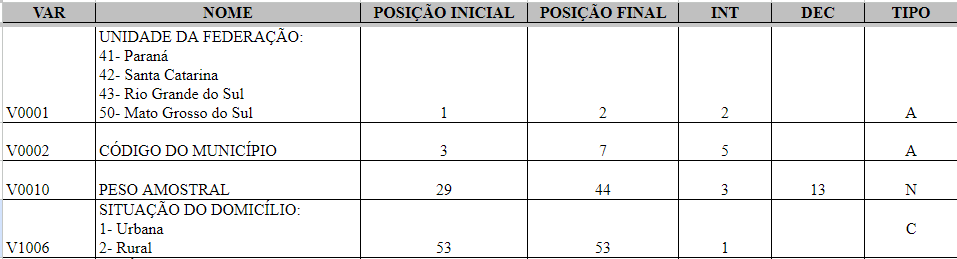
\includegraphics[width=\textwidth]{files/img/layout amostra domicilios 2010.png}
    \caption{Recorte da planilha de \textit{layout} da pesquisa de domicílios do Censo Demográfico de 2010. Fonte: Dados do Autor (2023).}
    \label{fig:layout-domi}
\end{figure}

    Variáveis padrões contidas nas pesquisas são as referentes à localização geográfica como município, UF e área de ponderação, assim como o peso amostral, que por sua vez é uma medida de representatividade daquela resposta dentro do escopo da pesquisa.

    Os arquivos de microdados ficam disponíveis através da URL <\url{www.ibge.gov.br/estatisticas/sociais/trabalho/22827-censo-demografico-2022.html?edicao=37225&t=microdados}>, separados por Estado e por Censo, hoje\footnote{Considerando o último acesso em novembro de 2023.} estando disponíveis os microdados Censos de 2000 e 2010 no \textit{website}. Com o intuito de facilitar o processo de baixar os arquivos, foi codificado um \textit{script python}\footnote{Código completo no arquivo download-arquivos-microdados.ipynb, disponível em: <\url{github.com/GDevigili/TCC-IBGE/blob/main/src/notebooks/download-arquivos-microdados.ipynb}>} para tal, que realiza o \textit{download} de todos os arquivos \verb|.zip|, descompacta eles e então os renomeia, de modo a padronizar os nomes dos arquivos de ambas pesquisas e separar as diferentes amostras, além de separar arquivos de dados dos arquivos auxiliares que estão inclusos nos diretórios compactados. Vale ressaltar que os arquivos não processados não foram incluídos no repositório por conta do limite máximo de 100 megabytes (MB) que o \textit{Github} impõe para os arquivos.

    Após extraídos os \verb|zip|s, tem-se uma coleção de arquivos de texto (de extensão \verb|.txt|) contendo os microdados codificados como na figura \ref{fig:exemplo-microdado}. Para transformá-los em dados utilizáveis, os microdados precisam ser associados aos respectivos valores, descritos no arquivo de \textit{layout}.

    Inicialmente, tentou-se fazer tal ``tradução'' via \textit{python}\footnote{Código completo no arquivo translate-microdata.ipynb, disponível em <\url{github.com/GDevigili/TCC-IBGE/blob/main/src/notebooks/old-notebooks/2-translate-microdata.ipynb}>}, manualmente programando tal a associação dos IDs com suas respectivas \textit{labels}. Primeiramente destrinchando o arquivo de descrição das variáveis em pares chave-valor e dividindo os números dos microdados em colunas de acordo com as respectivas posições inicial e final, armazenando ambos os resultados deste pré-processamento em \verb|DataFrame| da biblioteca \verb|pandas|. Tendo em mãos os objetos necessários, foi iterado através de cada linha e coluna, substituindo os identificadores por suas respectivas \textit{labels}.

    Porém, o custo computacional de se processar os dados dessa forma, ainda mais utilizando uma linguagem \textit{python}, conhecida por um tempo de execução elevado, além da presença de \textit{bugs} no código devido ao funcionamento de algumas estruturas de dados da \verb|pandas|, foi optado por realizar o mesmo trabalho utilizando o \textit{software Stata} (em sua versão 18.0), que possui funções já implementadas para o processamento de arquivos como os do IBGE.

    Com comandos da linguagem própria do \textit{Stata}, é possível fazer a mesma associação de identificadores e labels com alguns poucos comandos, para então gerar um arquivo de dados de extenção \verb|.dta| que posteriormente poderá ser utilizado como \textit{dataset}. Por exemplo, no \textit{Listing} \ref{lst:do-file-sample} definimos a posição das variáveis, sua tipagem, respectivas \textit{labels} e possíveis valores, nos casos de colunas categóricas, ou formatação, em caso de colunas numéricas.

    % De modo a preparar os microdados para que estes possam ser utilizados, foi utilizado o \textit{software} Stata (em sua versão 18.0) para associar os IDs e respectivos valores descritos no arquivo de \textit{layout} e então gerar um arquivo de dados que posteriormente poderá ser utilizado como \textit{dataset}. 
    % Com comandos do Stata é possível definir a posição em que se encontram as informações de cada variável, sua tipagem, suas \textit{labels} e respectivos pares chave e valor, para então o arquivo de dados ser processado, que é exemplificado pelo \textit{Listing} \ref{lst:do-file-sample} a seguir:

\begin{lstlisting}[float = ht, label={lst:do-file-sample},language=Stata, caption=Exemplo de comandos Stata utilizados para``traduzir'' os microdados.]
* Define as posições onde se encontram cada dado
quietly infix               ///
  byte		V1006		53-53		  ///
  double		V6204		82-84		///
using `"amostra_domicilios_2010_RJ.txt"', clear
* Define a formatação dos dados numéricos
* Neste caso,  o dado deve assumir a formatação 0000.0
format V6204 %04.1f
* Define as labels para os dados
label var V1006		`"SITUAÇÃO DO DOMICÍLIO"'
label var V6204		`"DENSIDADE DE MORADOR / DORMITÓRIO  "'
* Define os pares chave-valor para cada variável
label define V1006_lbl 1 `" Urbana"', add
label define V1006_lbl 2 `" Rural"', add
* Associa os valores da variável V1006 com os pares chave-valor armazenados em V1006_lbl
label values V1006 V1006_lbl
\end{lstlisting}

    O código exemplificado nada mais é que um pequeno recorte do arquivo\footnote{Arquivo\ amostra\_domicilios\_2010.do, disponível em <\url{https://github.com/GDevigili/TCC-IBGE/blob/main/src/do-files/amostra_domicilios_2010.do}>} completo da pesquisa de domicílios, que conta com 76 variáveis e mais de 6 mil \textit{labels}, em sua maioria referentes à localização geográfica da coleta da amostra, já que estão inclusos mais de 5 mil municípios e 500 microrregiões.

    Para não ser necessário definir manualmente cada uma das variáveis, aproveitou-se parte do código que seria descartada na tentativa de realizar a ``tradução'' dos microdados via \textit{python} e se utilizou do processamento da tabela de \textit{layout} para gerar um \textit{DataFrame} contendo os pares chave-valor utilizados para mapear via comando \verb|label define| as possíveis \textit{labels} de cada uma das colunas utilizando um \textit{script} que itera sobre a tabela processada.

    Além disso, como os códigos de município, micro e mesorregião ficam em planilhas auxiliares, foi optado por utilizar dos dados coletados via API para associar os respectivos códigos no \textit{Dofile} que seria executado no \textit{Stata} para gerar o conjunto de dados. A única transformação necessária foi o uso de uma coluna auxiliar que juntava o código da UF com os códigos de município e regiões, já que a API utiliza chaves concatenadas como identificadores.

    Após gerado o \textit{Dofile} através do \textit{script} \textit{python} descrito acima, só é necessário carregar o arquivo no \textit{Stata} e executá-lo, por fim salvando o novo arquivo de dados.
    
    % Como facilitador para tal associação de pares chave-valor, foi desenvolvido um código \textit{python}\footnote{Código disponível em <\url{https://github.com/GDevigili/DW-IBGE/blob/main/src/notebooks/gera-script-stata.ipynb}>.} que gera um \textit{script} para ser utilizado pelo Stata para o processamento  ``tradução'' dos microdados. 
   
    % Primeiramente, por meio das colunas de posição inicial e final, foram mapeados os caracteres que representam cada uma das variáveis do conjunto de dados, então foi adicionada a formatação adequada para os dados numéricos com o comando \verb|format|. Posteriormente são definidos os nomes das colunas com o comando \verb|label define| e então associados os pares chave-valor, extraídos de um \verb|DataFrame| pré processado com os dados presentes no arquivo de \textit{layout}. Os valores correspondentes aos municípios, microrregiões, mesorregiões e regiões metropolitanas se encontram em arquivos auxiliares, porém foi optado por utilizar a própria API de localidades para obter os respectivos valores já que o trabalho para a extração de dados já havia sido realizado anteriormente.


\chapter{Estudo de Caso}